\section{Industrial design}

In this section, the industrial design will be explained and especially shown with pictures to have an idea of how the product will look. The design part was done by the ECAL student. The indutrial designer presented different solutions, they were then discussed together with the other member of the group. The solutions were also presented to the nurses and some old people to define which one is the more understandable and easy to use.

\subsection{Tablet}


The design of the tablet is shown in the figure \ref{fig:vesta design}.

\begin{figure}[!htb]
    \centering
    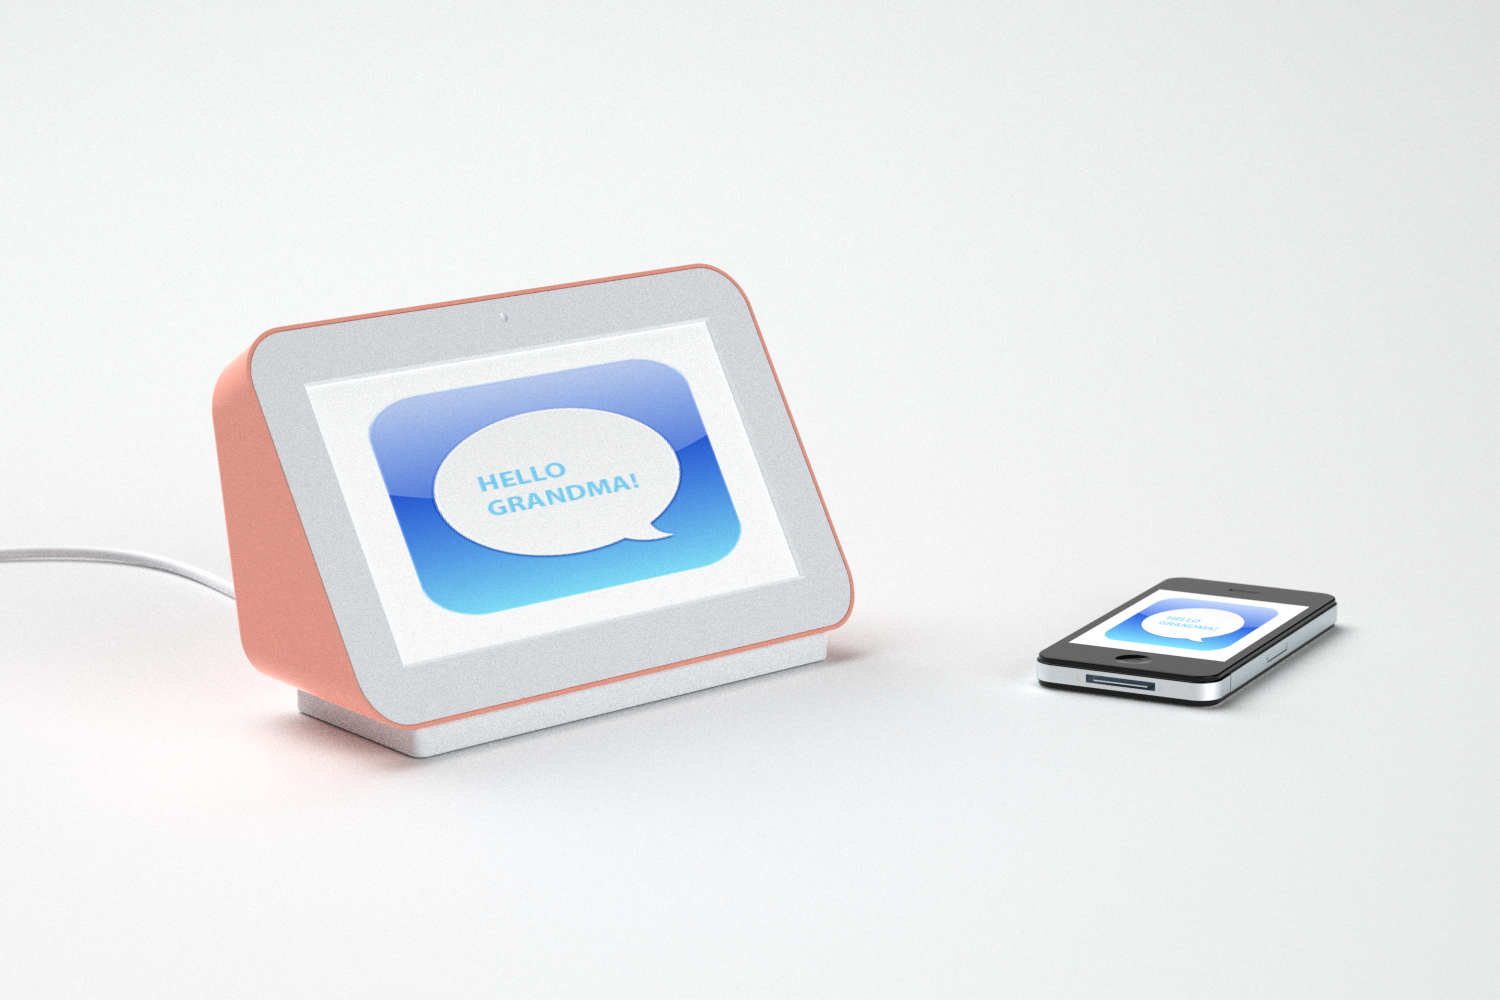
\includegraphics[width=0.9\textwidth,keepaspectratio]{chap/designFig/VestaRender4.png}
    \caption{Vesta tablet design}
    \label{fig:vesta design}
\end{figure}


\subsection{Charging station}

\begin{figure}[!htb]
    \centering
    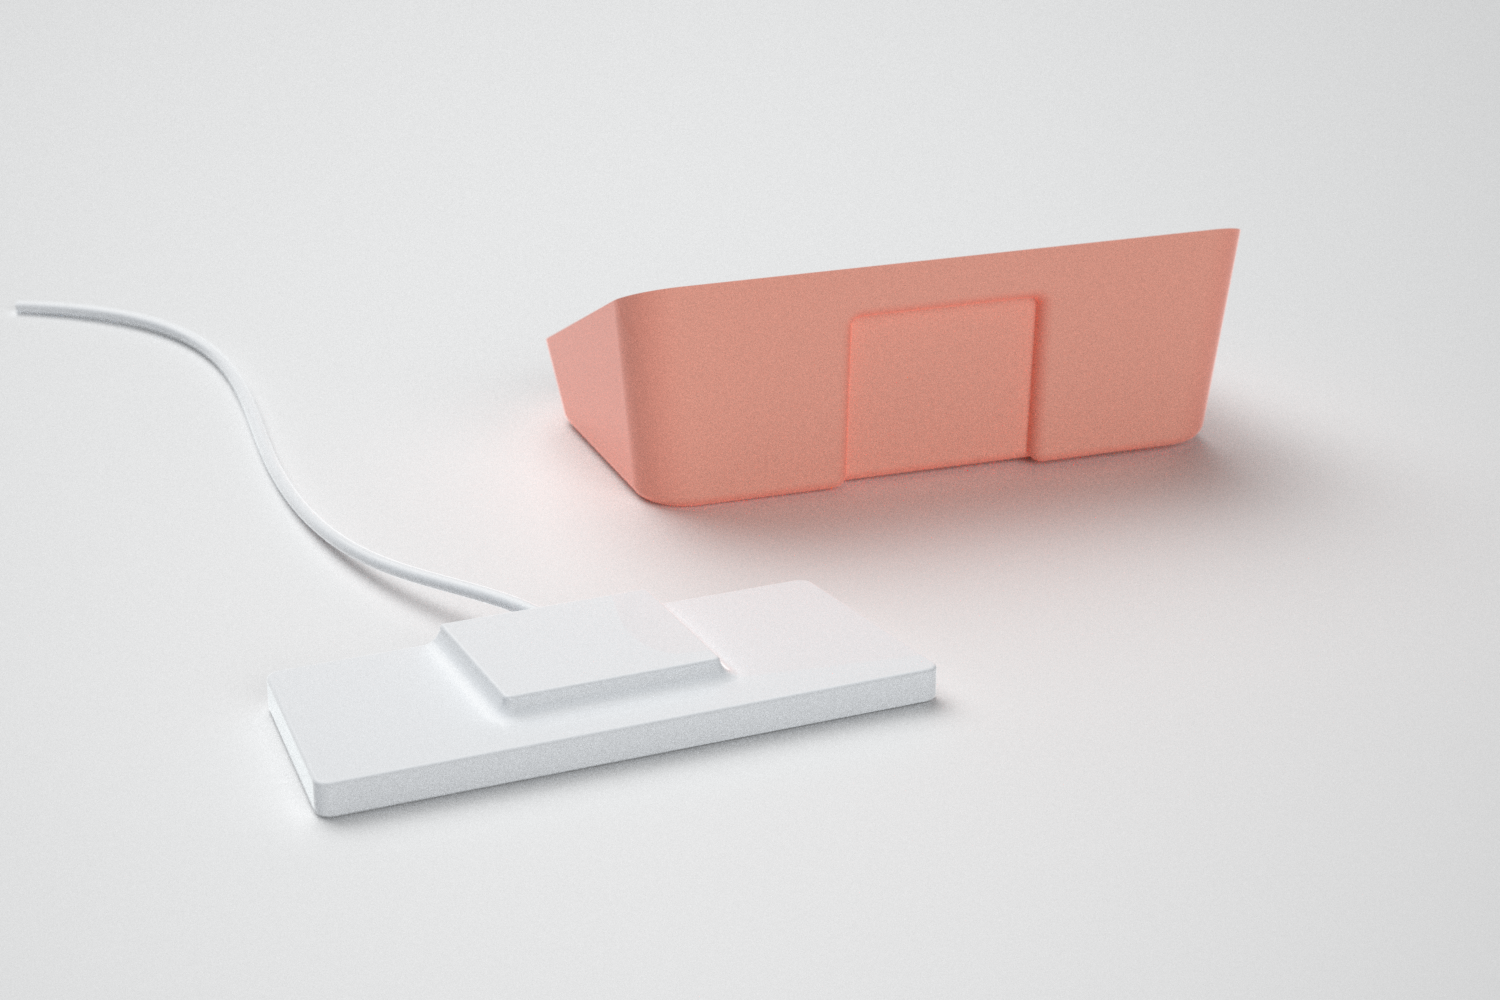
\includegraphics[width=0.9\textwidth,keepaspectratio]{chap/designFig/VisioRender7.png}
    \caption{Charging station}
    \label{fig:charging station}
\end{figure}

\clearpage

\subsection{Software design}

The graphical interface of the software is shown in the figure \ref{fig:soft design}.

\begin{figure}[!htb]
    \centering
    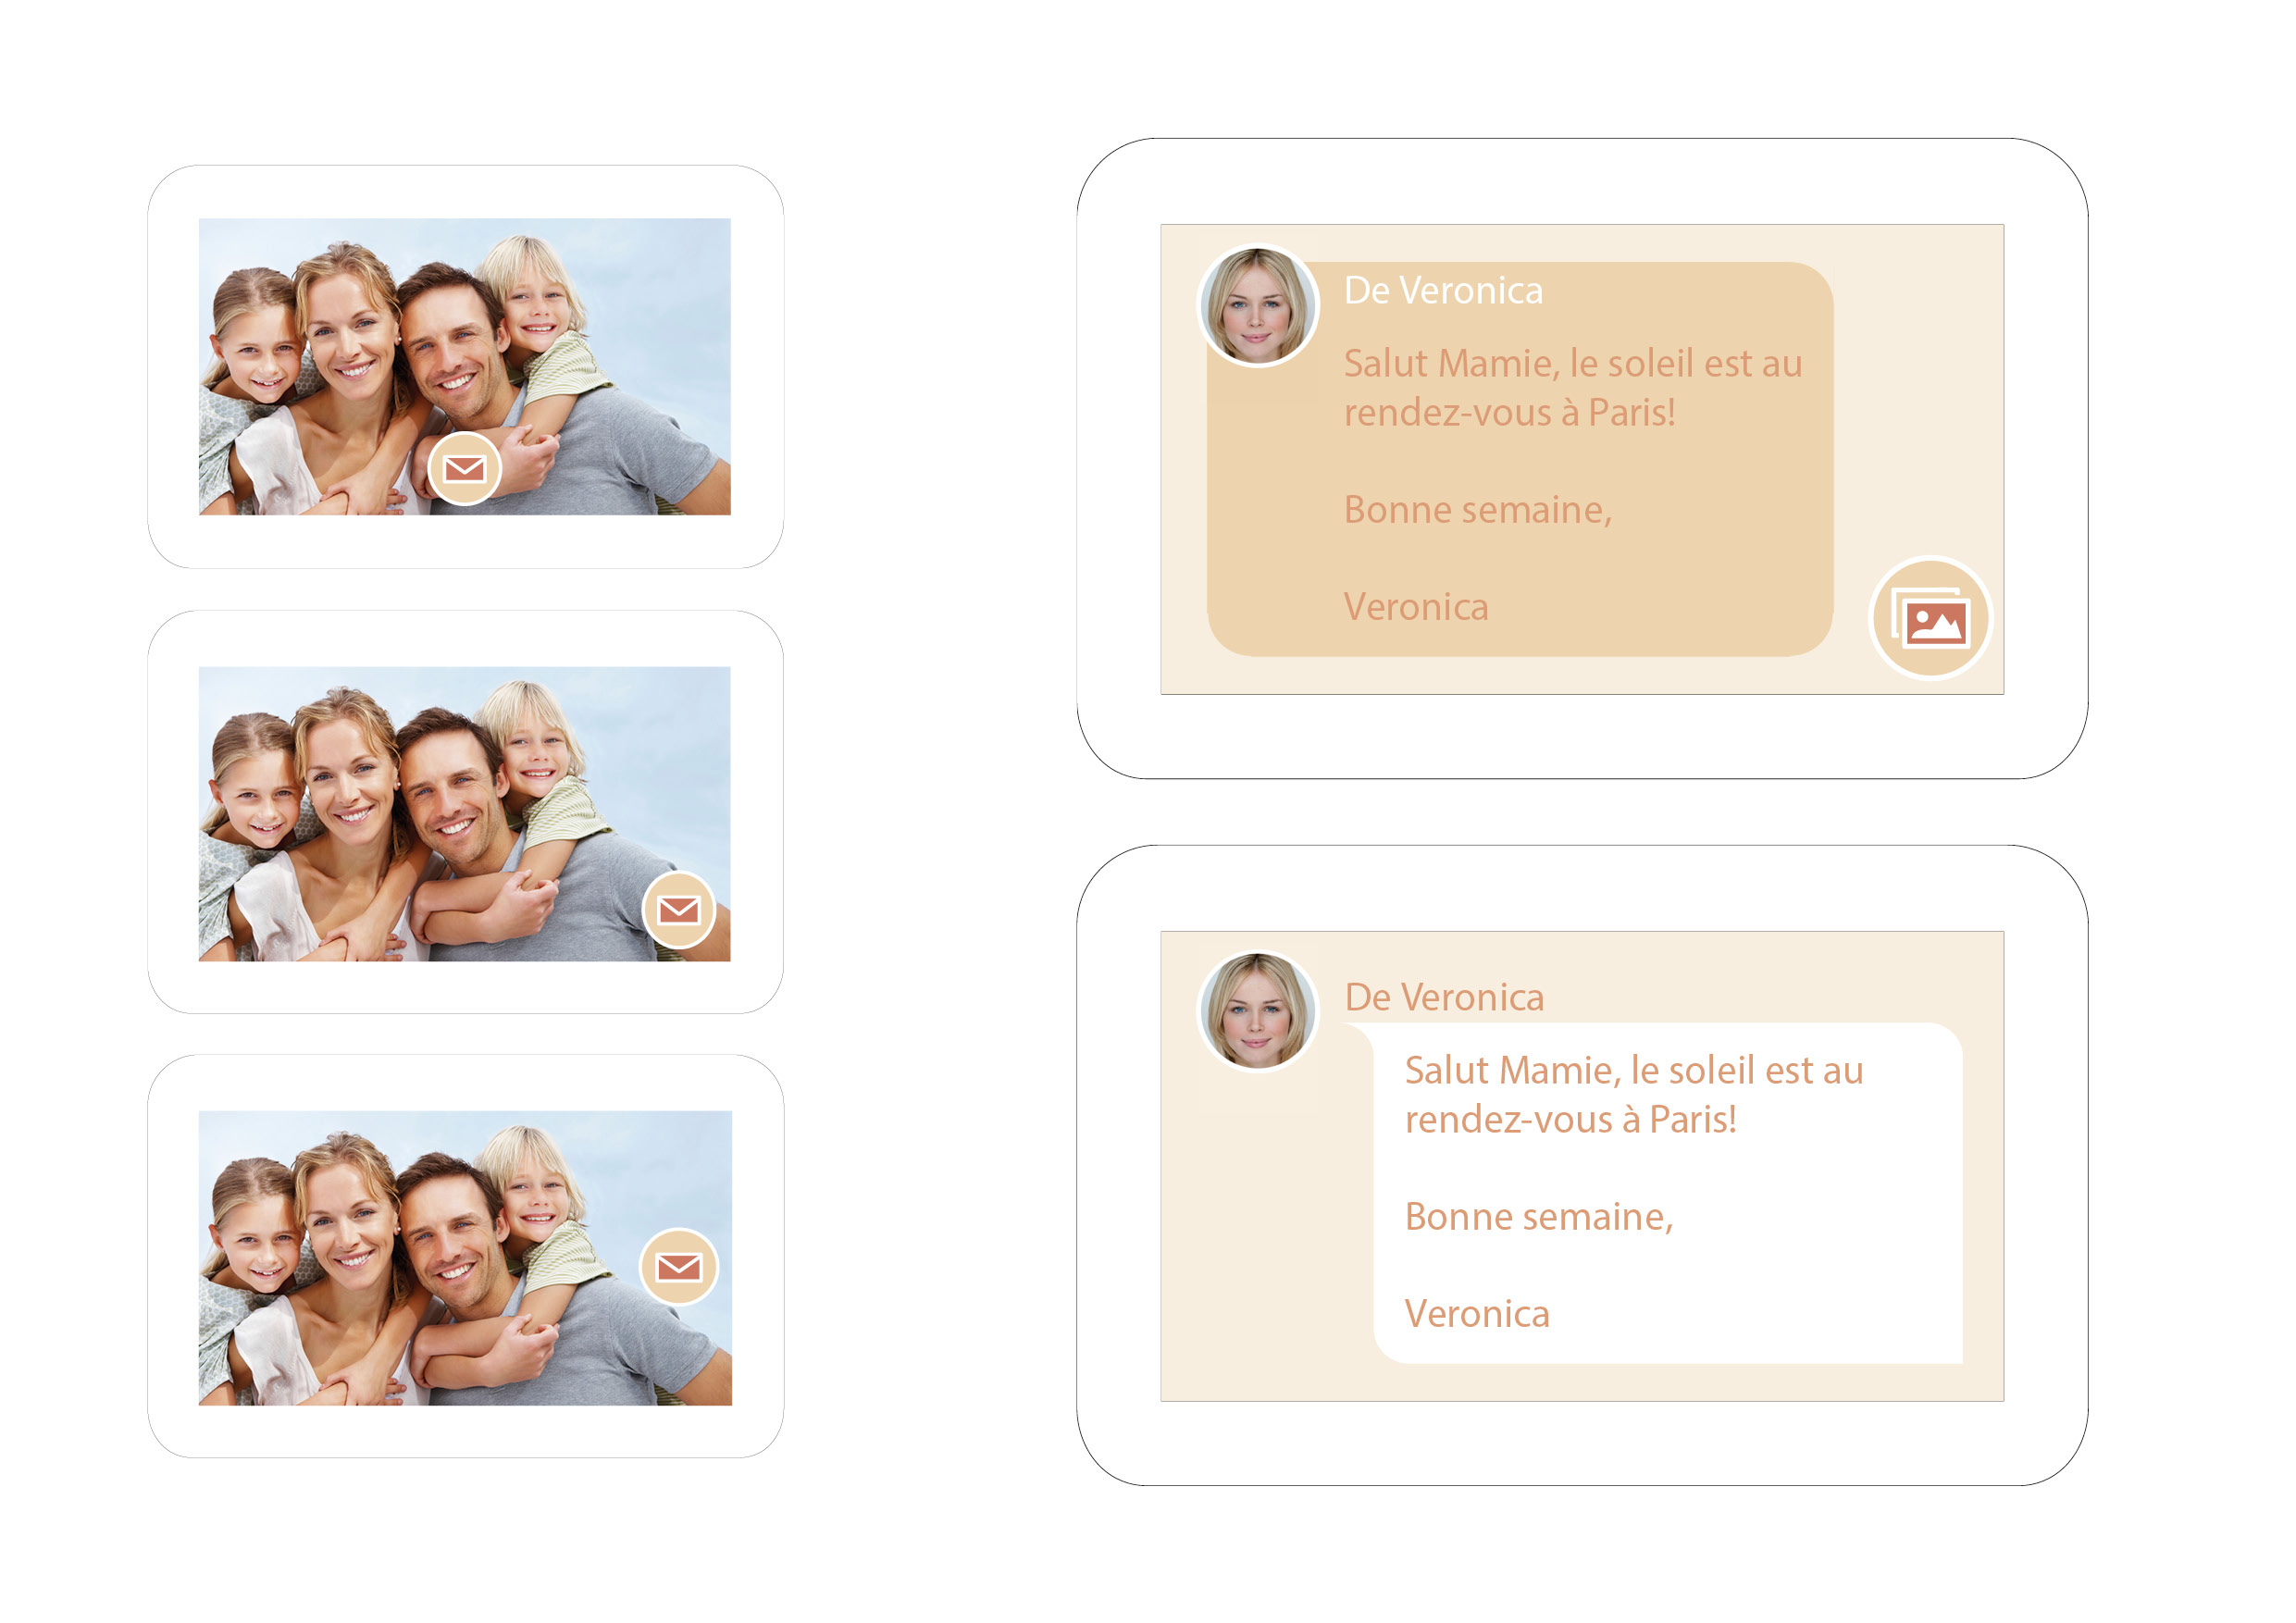
\includegraphics[width=0.9\textwidth,keepaspectratio]{chap/designFig/vesta_design.jpg}
    \caption{Software design}
    \label{fig:soft design}
\end{figure}
